\documentclass[tikz, border=4pt]{standalone}
\usepackage{amsmath}
\usetikzlibrary{arrows.meta}

% Computational domain and boundary conditions of laminar/cavity3d, also used
% by laminar/cavity3dBenchmark. Render the PDF and the SVG used by the user
% guide next to this file with
%   pdflatex cavity3dDomain.tex && pdf2svg cavity3dDomain.pdf cavity3dDomain.svg

\begin{document}
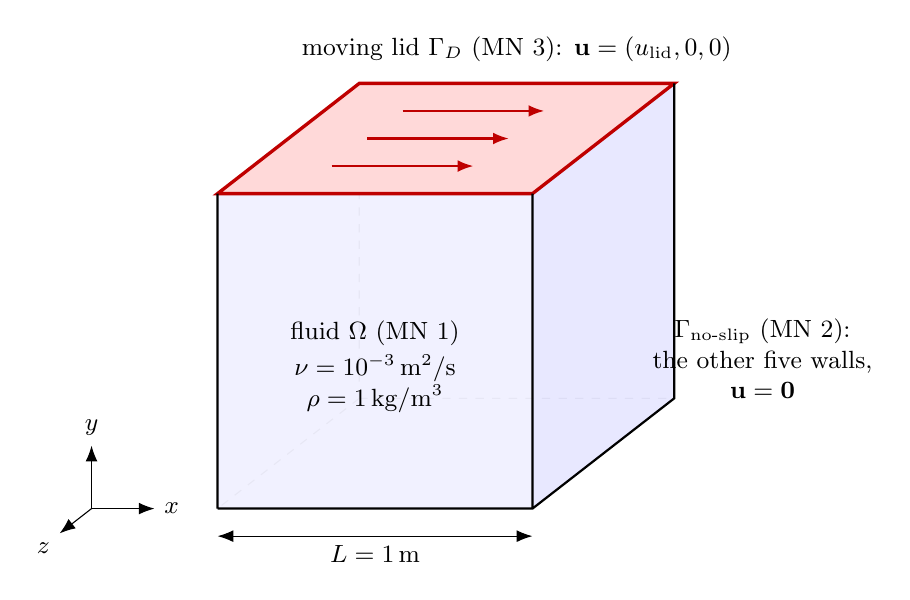
\begin{tikzpicture}[
    >={Latex[length=2mm]},
    x={(1cm,0cm)}, y={(0cm,1cm)}, z={(-0.45cm,-0.35cm)},
    label/.style={font=\small, align=center},
  ]
  \def\L{4}

  % hidden edges
  \draw[black!40, dashed] (0,0,0) -- (\L,0,0) (0,0,0) -- (0,\L,0) (0,0,0) -- (0,0,\L);

  % walls at rest (MN 2): the visible faces, without the lid
  \fill[blue!6, opacity=0.9] (0,0,\L) -- (\L,0,\L) -- (\L,\L,\L) -- (0,\L,\L) -- cycle;
  \fill[blue!10, opacity=0.9] (\L,0,0) -- (\L,0,\L) -- (\L,\L,\L) -- (\L,\L,0) -- cycle;

  % moving lid (MN 3) at y = L
  \fill[red!15] (0,\L,0) -- (\L,\L,0) -- (\L,\L,\L) -- (0,\L,\L) -- cycle;
  \draw[very thick, red!75!black] (0,\L,0) -- (\L,\L,0) -- (\L,\L,\L) -- (0,\L,\L) -- cycle;
  \foreach \zz in {0.25,0.5,0.75}
    \draw[->, thick, red!75!black] (0.25*\L,\L,\zz*\L) -- ++(0.45*\L,0,0);

  % visible edges
  \draw[thick] (0,0,\L) -- (\L,0,\L) -- (\L,0,0) -- (\L,\L,0)
               (0,0,\L) -- (0,\L,\L) (\L,0,\L) -- (\L,\L,\L);

  % labels
  \node[label, above] at (0.5*\L,\L+0.15,0)
    {moving lid $\Gamma_D$ (MN 3): $\mathbf{u} = (u_\text{lid}, 0, 0)$};
  \node[label] at (0.5*\L,0.45*\L,\L)
    {fluid $\Omega$ (MN 1)\\[2pt] $\nu = 10^{-3}\,\mathrm{m^2/s}$\\ $\rho = 1\,\mathrm{kg/m^3}$};
  \node[label, right] at (\L+0.5,0.3*\L,0.5*\L)
    {$\Gamma_{\mathrm{no\text{-}slip}}$ (MN 2):\\ the other five walls,\\ $\mathbf{u} = \mathbf{0}$};

  % dimensions
  \draw[<->, thin] (0,-0.35,\L) -- node[below, font=\small] {$L = 1\,\mathrm{m}$} (\L,-0.35,\L);

  % coordinate system
  \begin{scope}[shift={(-1.6,0,\L)}]
    \draw[->] (0,0,0) -- (0.8,0,0) node[right, font=\small] {$x$};
    \draw[->] (0,0,0) -- (0,0.8,0) node[above, font=\small] {$y$};
    \draw[->] (0,0,0) -- (0,0,0.9) node[below left, font=\small] {$z$};
  \end{scope}
\end{tikzpicture}
\end{document}
